% Options for packages loaded elsewhere
\PassOptionsToPackage{unicode}{hyperref}
\PassOptionsToPackage{hyphens}{url}
%
\documentclass[
  9pt,
  ignorenonframetext,
]{beamer}
\usepackage{pgfpages}
\setbeamertemplate{caption}[numbered]
\setbeamertemplate{caption label separator}{: }
\setbeamercolor{caption name}{fg=normal text.fg}
\beamertemplatenavigationsymbolsempty
% Prevent slide breaks in the middle of a paragraph
\widowpenalties 1 10000
\raggedbottom
\setbeamertemplate{part page}{
  \centering
  \begin{beamercolorbox}[sep=16pt,center]{part title}
    \usebeamerfont{part title}\insertpart\par
  \end{beamercolorbox}
}
\setbeamertemplate{section page}{
  \centering
  \begin{beamercolorbox}[sep=12pt,center]{part title}
    \usebeamerfont{section title}\insertsection\par
  \end{beamercolorbox}
}
\setbeamertemplate{subsection page}{
  \centering
  \begin{beamercolorbox}[sep=8pt,center]{part title}
    \usebeamerfont{subsection title}\insertsubsection\par
  \end{beamercolorbox}
}
\AtBeginPart{
  \frame{\partpage}
}
\AtBeginSection{
  \ifbibliography
  \else
    \frame{\sectionpage}
  \fi
}
\AtBeginSubsection{
  \frame{\subsectionpage}
}

\usepackage{amsmath,amssymb}
\usepackage{lmodern}
\usepackage{iftex}
\ifPDFTeX
  \usepackage[T1]{fontenc}
  \usepackage[utf8]{inputenc}
  \usepackage{textcomp} % provide euro and other symbols
\else % if luatex or xetex
  \usepackage{unicode-math}
  \defaultfontfeatures{Scale=MatchLowercase}
  \defaultfontfeatures[\rmfamily]{Ligatures=TeX,Scale=1}
\fi
% Use upquote if available, for straight quotes in verbatim environments
\IfFileExists{upquote.sty}{\usepackage{upquote}}{}
\IfFileExists{microtype.sty}{% use microtype if available
  \usepackage[]{microtype}
  \UseMicrotypeSet[protrusion]{basicmath} % disable protrusion for tt fonts
}{}
\makeatletter
\@ifundefined{KOMAClassName}{% if non-KOMA class
  \IfFileExists{parskip.sty}{%
    \usepackage{parskip}
  }{% else
    \setlength{\parindent}{0pt}
    \setlength{\parskip}{6pt plus 2pt minus 1pt}}
}{% if KOMA class
  \KOMAoptions{parskip=half}}
\makeatother
\usepackage{xcolor}
\newif\ifbibliography
\setlength{\emergencystretch}{3em} % prevent overfull lines
\setcounter{secnumdepth}{-\maxdimen} % remove section numbering


\providecommand{\tightlist}{%
  \setlength{\itemsep}{0pt}\setlength{\parskip}{0pt}}\usepackage{longtable,booktabs,array}
\usepackage{calc} % for calculating minipage widths
\usepackage{caption}
% Make caption package work with longtable
\makeatletter
\def\fnum@table{\tablename~\thetable}
\makeatother
\usepackage{graphicx}
\makeatletter
\def\maxwidth{\ifdim\Gin@nat@width>\linewidth\linewidth\else\Gin@nat@width\fi}
\def\maxheight{\ifdim\Gin@nat@height>\textheight\textheight\else\Gin@nat@height\fi}
\makeatother
% Scale images if necessary, so that they will not overflow the page
% margins by default, and it is still possible to overwrite the defaults
% using explicit options in \includegraphics[width, height, ...]{}
\setkeys{Gin}{width=\maxwidth,height=\maxheight,keepaspectratio}
% Set default figure placement to htbp
\makeatletter
\def\fps@figure{htbp}
\makeatother

\usepackage{bm}
\usepackage{lmodern}
\usetheme{Madrid}
\usepackage{appendixnumberbeamer}
\setbeamertemplate{itemize items}[square]
\settowidth{\leftmargini}{\usebeamertemplate{itemize item}}
\addtolength{\leftmargini}{\labelsep}
\beamertemplatenavigationsymbolsempty % don't show the navigation bar
\definecolor{emph2}{RGB}{230,160,25}       % HTF orange for emphasis
\definecolor{titles}{RGB}{48,57,172}        % Light blue for the titles
\definecolor{structural}{RGB}{6,35, 101}   % Dark blue for the template
\setbeamercolor{structure}{fg=structural} % titles, itemize, itemize, etc
\setbeamercolor{block title}{bg=white, fg=titles}
\setbeamercolor{item}{fg=titles}
\setbeamerfont{title}{size=\huge}
\setbeamerfont{subtitle}{size=\normalsize}
\setbeamerfont{frametitle}{size=\huge}
\setbeamerfont{author}{size=\large}
\setbeamerfont{institute}{size=\normalsize}
\setbeamerfont{date}{size=\small}
\setbeamerfont{frame number in foot}{size=\scriptsize}
\makeatletter
\makeatother
\makeatletter
\makeatother
\makeatletter
\@ifpackageloaded{caption}{}{\usepackage{caption}}
\AtBeginDocument{%
\ifdefined\contentsname
  \renewcommand*\contentsname{Table of contents}
\else
  \newcommand\contentsname{Table of contents}
\fi
\ifdefined\listfigurename
  \renewcommand*\listfigurename{List of Figures}
\else
  \newcommand\listfigurename{List of Figures}
\fi
\ifdefined\listtablename
  \renewcommand*\listtablename{List of Tables}
\else
  \newcommand\listtablename{List of Tables}
\fi
\ifdefined\figurename
  \renewcommand*\figurename{Figure}
\else
  \newcommand\figurename{Figure}
\fi
\ifdefined\tablename
  \renewcommand*\tablename{Table}
\else
  \newcommand\tablename{Table}
\fi
}
\@ifpackageloaded{float}{}{\usepackage{float}}
\floatstyle{ruled}
\@ifundefined{c@chapter}{\newfloat{codelisting}{h}{lop}}{\newfloat{codelisting}{h}{lop}[chapter]}
\floatname{codelisting}{Listing}
\newcommand*\listoflistings{\listof{codelisting}{List of Listings}}
\makeatother
\makeatletter
\@ifpackageloaded{caption}{}{\usepackage{caption}}
\@ifpackageloaded{subcaption}{}{\usepackage{subcaption}}
\makeatother
\makeatletter
\@ifpackageloaded{tcolorbox}{}{\usepackage[many]{tcolorbox}}
\makeatother
\makeatletter
\@ifundefined{shadecolor}{\definecolor{shadecolor}{rgb}{.97, .97, .97}}
\makeatother
\makeatletter
\makeatother
\ifLuaTeX
  \usepackage{selnolig}  % disable illegal ligatures
\fi
\IfFileExists{bookmark.sty}{\usepackage{bookmark}}{\usepackage{hyperref}}
\IfFileExists{xurl.sty}{\usepackage{xurl}}{} % add URL line breaks if available
\urlstyle{same} % disable monospaced font for URLs
\hypersetup{
  pdftitle={Computational Statistics II},
  pdfauthor={Tommaso Rigon},
  hidelinks,
  pdfcreator={LaTeX via pandoc}}

\title{Computational Statistics II}
\subtitle{Unit A.1: Metropolis-Hastings and Gibbs sampling}
\author{Tommaso Rigon}
\date{}
\institute{Unimib}

\begin{document}
\frame{\titlepage}
\ifdefined\Shaded\renewenvironment{Shaded}{\begin{tcolorbox}[frame hidden, sharp corners, boxrule=0pt, interior hidden, borderline west={3pt}{0pt}{shadecolor}, enhanced, breakable]}{\end{tcolorbox}}\fi

\begin{frame}{Unit A.1}
\protect\hypertarget{unit-a.1}{}
\begin{block}{Topics}
\protect\hypertarget{topics}{}
\begin{itemize}
\tightlist
\item
  Markov Chain Monte Carlo (MCMC)
\item
  The Metropolis--Hastings algorithm
\item
  The Gibbs sampling algorithm
\item
  Writing clean and efficient \textbf{R} code
\end{itemize}
\end{block}

\begin{block}{Main references}
\protect\hypertarget{main-references}{}
\begin{itemize}
\tightlist
\item
  Robert, C. P., and Casella, G. (2004). Monte Carlo Statistical
  Methods. Springer.
\item
  Roberts, G. O., and Rosenthal, J. S. (2004). General state space
  Markov chains and MCMC algorithms. Probability Surveys, 1(1), 20--71.
\item
  Tierney, L. (1994). Markov chains for exploring posterior
  distributions. Annals of Statistics, 22(4), 1701-176.
\end{itemize}

Associated \textbf{R} code is available on the website of the course.
\end{block}
\end{frame}

\begin{frame}{Bayesian computations}
\protect\hypertarget{bayesian-computations}{}
\begin{itemize}
\item
  Over the past 30 years, Markov Chain Monte Carlo methods (MCMC)
  methods have \textbf{revolutionized} Bayesian statistics.
\item
  Bayesian computational statistics is nowadays a lively and mature
  research field, compared to the early days. Still, there are several
  open questions.
\end{itemize}

\begin{quote}
``Arguably the biggest challenge is in computation. If MCMC is no longer
viable for the problems people want to address, then what is the role of
INLA, of variational methods, of ABC approaches?'' \textbf{Alan Gelfand}
(ISBA bullettin, 2011)
\end{quote}

\begin{itemize}
\tightlist
\item
  \url{https://www.stat.berkeley.edu/~aldous/157/Papers/Bayesian_open_problems.pdf}
\end{itemize}
\end{frame}

\begin{frame}[fragile]{Bayesian inference (recap)}
\protect\hypertarget{bayesian-inference-recap}{}
\begin{itemize}
\item
  Let \(\bm{X}\) be the data, following some distribution
  \(\pi(\bm{X} \mid \bm{\theta})\), i.e.~the \textbf{likelihood}, with
  \(\bm{\theta} \in \Theta \subseteq \mathbb{R}^p\) being an unknown set
  of parameters.
\item
  Let \(\pi(\bm{\theta})\) be the \textbf{prior distribution} associated
  to \(\bm{\theta}\).
\item
  In Bayesian analysis, inference is based on the \textbf{posterior
  distribution} for \(\bm{\theta}\), defined as \[
  \pi(\bm{\theta} \mid \bm{X}) = \frac{\pi(\bm{\theta}) \pi(\bm{X} \mid \bm{\theta})}{\int_\Theta\pi(\bm{\theta}) \pi(\bm{X} \mid \bm{\theta}) \mathrm{d} \bm{\theta}}.
  \]
\item
  The \textbf{normalizing constant}, i.e.~the above integral, is often
  \textbf{intractable} \(\implies\) no analytical solutions, beyond
  conjugate cases.
\item
  Numerical approximations of
  \(\int_\Theta\pi(\bm{\theta}) \pi(\bm{X} \mid \bm{\theta}) \mathrm{d} \bm{\theta}\)
  are highly unstable, especially in high dimensions \(\implies\) the
  \texttt{integrate} \textbf{R} function will not work in most cases.
\end{itemize}
\end{frame}

\begin{frame}{Bayesian inference using sampling}
\protect\hypertarget{bayesian-inference-using-sampling}{}
\begin{itemize}
\item
  It is sometimes possible to \textbf{sample} from the posterior
  distribution even without knowing the normalizing constant.
\item
  If we can get \textbf{random samples}
  \(\bm{\theta}^{(1)}, \dots,\bm{\theta}^{(R)}\) from the posterior
  distribution, then we can approximate any functional of interest, i.e.
  \[
  \mathbb{E}(g(\bm{\theta}) \mid \bm{X}) \approx \frac{1}{R}\sum_{r=1}^R g(\bm{\theta}^{(r)}).
  \]
\item
  If \(\bm{\theta}^{(1)}, \dots,\bm{\theta}^{(R)}\) were
  \textbf{independent} samples from the posterior distribution, this
  approximation would be called \textbf{Monte Carlo integration}.
\item
  Monte Carlo integration is justified by the \textbf{law of large
  numbers}.
\item
  In this course, we will consider samples
  \(\bm{\theta}^{(1)}, \dots,\bm{\theta}^{(R)}\) that are
  \textbf{dependent} and follow a Markov Chain \(\implies\) Markov Chain
  Monte Carlo (MCMC).
\end{itemize}
\end{frame}

\begin{frame}{Markov chains}
\protect\hypertarget{markov-chains}{}
\begin{itemize}
\item
  A sequence \(\bm{Y}^{(0)}, \bm{Y}^{(1)}, \dots, \bm{Y}^{(R)}\) of
  random elements is a \textbf{Markov chain} if \[
  \mathbb{P}(\bm{Y}^{(r + 1)} \in A \mid \bm{y}^{(0)}, \dots, \bm{y}^{(r)}) = \mathbb{P}(\bm{Y}^{(r + 1)} \in A \mid\bm{y}^{(r)}). 
  \]
\item
  In other words, the conditional distribution of \(\bm{Y}^{(r + 1)}\)
  given \(\bm{y}^{(0)}, \dots, \bm{y}^{(r)}\) is the same as the
  conditional distribution of \(\bm{Y}^{(r + 1)}\) given
  \(\bm{y}^{(r)}\), called \textbf{transition kernel}.
\item
  Given an initial condition \(\bm{y}^{(0)}\) a Markov chain is fully
  characterized by its transition kernel, which we assume does not
  depend on \(r\) (\textbf{homogeneity}).
\item
  In continuous cases, the transition kernel is identified by a
  \textbf{conditional density}, denoted with \[
  k(\bm{y}^{(r+1)} \mid \bm{y}^{(r)}).
  \]
\item
  When the sample space is finite, the transition kernel is a
  \textbf{transition matrix}, say \(P\).
\end{itemize}
\end{frame}

\begin{frame}{Example: AR(1)}
\protect\hypertarget{example-ar1}{}
\begin{itemize}
\item
  \textbf{Autoregressive} processes provide a simple illustration of
  \textbf{Markov chains} on continuous state-space.
\item
  Let \(Y^{(0)} \sim N(30, 1)\) and let us define \[
  Y^{(r)} = \rho Y^{(r-1)} + \epsilon^{(r)}, \qquad \rho \in \mathbb{R},
  \] with the error terms \(\epsilon^{(r)}\) being iid according to a
  standard Gaussian \(\text{N}(0,1)\).
\item
  Then the sequence of \(Y^{(r)}\) forms indeed a Markov chain and the
  \textbf{transition density} is such that \[
  (y^{(r)} \mid y^{(r-1)})  \sim \text{N}(\rho y^{(r-1)}, 1).
  \]
\item
  If the parameter \(|\rho| < 1\) then the Markov chain has a more
  ``stable'' behaviour.
\end{itemize}
\end{frame}

\begin{frame}{Example: AR(1)}
\protect\hypertarget{example-ar1-1}{}
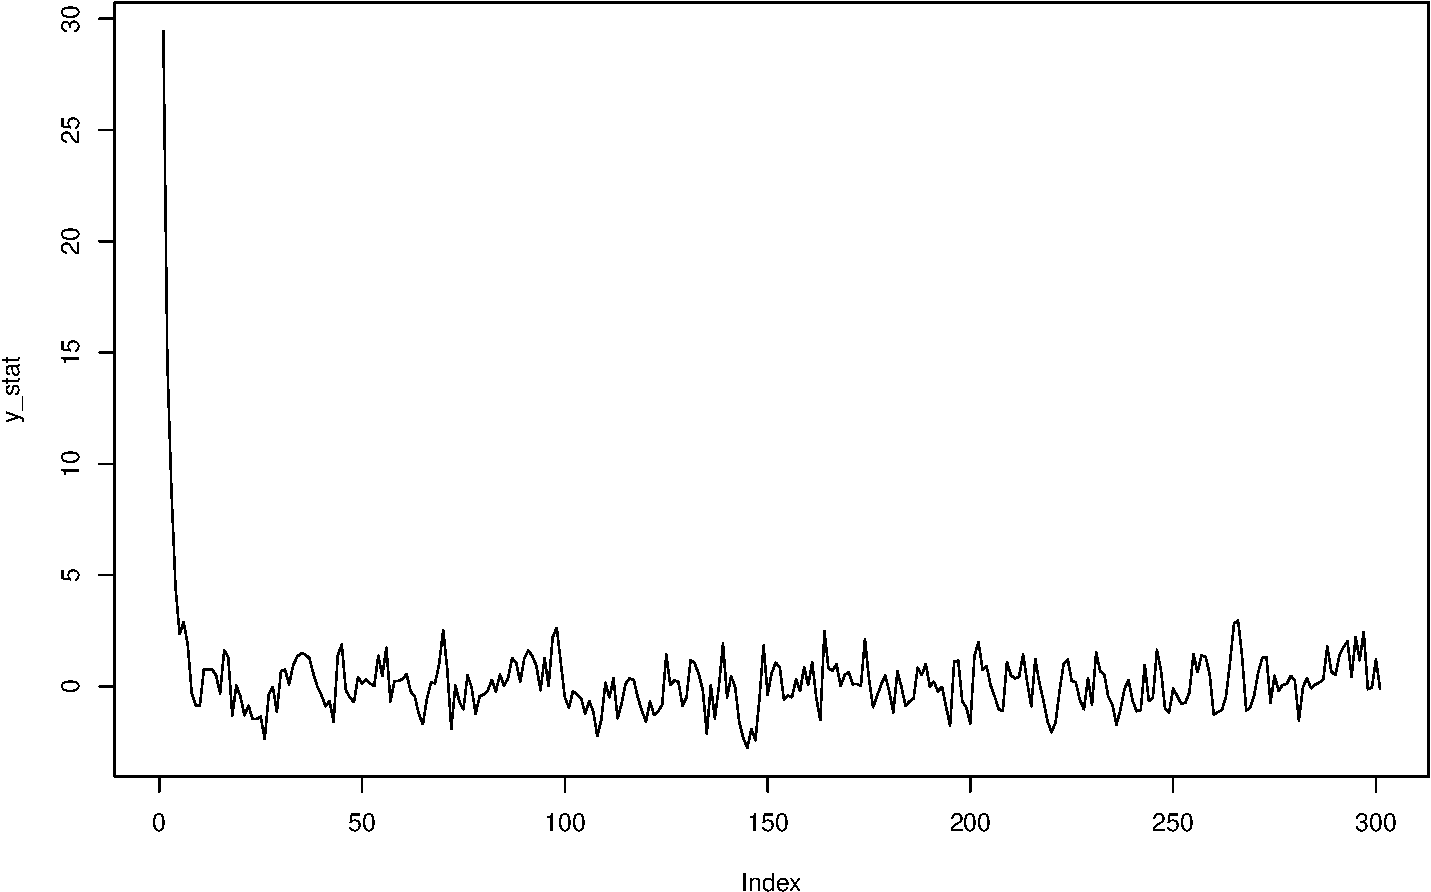
\includegraphics{un_A1_files/figure-beamer/unnamed-chunk-1-1.pdf}
\end{frame}

\begin{frame}{Invariant distribution}
\protect\hypertarget{invariant-distribution}{}
\begin{itemize}
\item
  An increased level of stability of a Markov chain occurs when the
  latter admits an \textbf{invariant} or \textbf{stationary} probability
  distribution.
\item
  A probability density \(\pi(\bm{y})\) is invariant for a Markov chain
  with kernel \(k\) if \[
  \pi(\bm{y}^*) = \int k(\bm{y}^* \mid \bm{y})\pi(\bm{y})\mathrm{d}\bm{y}.
  \]
\item
  This is to say that the \textbf{marginal} distributions of
  \(\bm{Y}^{(r)}\) and \(\bm{Y}^{(r + 1)}\) are the same and are equal
  to \(\pi(\bm{y})\), although \(\bm{Y}^{(r)}\) and \(\bm{Y}^{(r + 1)}\)
  remain \textbf{dependent}.
\item
  Roughly speaking, if a Markov chain admits a stationary distribution +
  some technical conditions, then for \(R\) large enough the chain
  ``stabilizes'' around the invariant law.
\item
  In the previous \(\textup{ar}(1)\) example the stationary distribution
  is \(\text{N}(0, 1 / (1 - \rho^2))\).
\end{itemize}
\end{frame}

\begin{frame}{Invariant distribution}
\protect\hypertarget{invariant-distribution-1}{}
\begin{itemize}
\item
  Not every Markov chain admits a stationary law. However, the Markov
  chains constructed for sampling purposes should always converge to an
  invariant distribution.
\item
  Indeed, in Markov Chain Monte Carlo the stationary distribution
  \(\pi(\bm{y})\) represents the \textbf{target density} from which we
  wish to simulate.
\item
  Then, we will make use of the following approximation \[
  \int g(\bm{y}) \pi(\bm{y})\mathrm{d}\bm{y} \approx \frac{1}{R}\sum_{r=1}^R g(\bm{y}^{(r)}),
  \] where \(\bm{y}^{(1)}, \dots, \bm{y}^{(R)}\) are generated according
  to a Markov chain, with \(\bm{y}^{(0)} \sim \pi(\bm{y})\).
\item
  How to construct a Markov chain that converges to the desired density
  \(\pi(\bm{y})\)?
\item
  Before delving into this key problem, let us briefly review the
  assumptions under which this approximation is a reasonable one.
\end{itemize}
\end{frame}

\begin{frame}{Regularity conditions}
\protect\hypertarget{regularity-conditions}{}
\begin{itemize}
\item
  We will consider Markov chains that are \textbf{irreducible},
  \textbf{aperiodic}, and \textbf{Harris recurrent}.
\item
  A rigorous presen \textbf{discrete case} to help the intuition.
\item
  For a more detailed treatment, see Chapter 6 of Robert and Casella
  (2004).
\item
  \textbf{Irreducibility}. The chain is irreducible if it does not ``get
  stuck'' in a local region of the sample space. In the discrete case
  the chain is irreducible if all states are connected.
\item
  \textbf{Aperiodicity}. The chain is aperiodic if it does not has any
  deterministic cycle.
\item
  \textbf{Harris recurrent}. The chain is (Harris) recurrent if it
  visits any region of the sample space ``sufficiently often''.
\end{itemize}
\end{frame}

\begin{frame}{Irreducibility}
\protect\hypertarget{irreducibility}{}
\begin{itemize}
\item
  The aforementioned properties are easy to formalize in the
  \textbf{discrete} setting, namely when the values of the Markov chain
  are \(Y^{(r)} \in \{1, 2,\dots\}\).
\item
  The \textbf{first passage time} is the first \(r\) for which the chain
  is equal to \(j\), namely: \[
  \tau_j = \inf\{r \ge 1 : Y^{(r)} = j\},
  \] where by convention we let \(\tau_j = \infty\) if
  \(Y^{(r)} \neq j\) for every \(r \ge 1\).
\item
  Moreover, let us denote the \textbf{probability of return} to \(j\) in
  a finite number of step, starting from \(j'\) \[
  \mathbb{P}(\tau_j < \infty \mid y^{(0)} = j').
  \]
\item
  Hence, the chain is \textbf{irreducible} if
  \(\mathbb{P}(\tau_j < \infty \mid y^{(0)} = j') > 0\) for all
  \(j, j' \in \mathbb{N}\).
\end{itemize}
\end{frame}



\end{document}
